\documentclass[11pt]{article}
\usepackage[a4paper,margin=1in]{geometry}
\usepackage{amsmath,amssymb}
\usepackage{tikz}
\usetikzlibrary{angles,quotes,calc}
\usepackage[hidelinks]{hyperref}
\hypersetup{pdftitle={Six circles in a rectangle},pdfauthor={Vamshi Jandhyala}}
\setlength{\parskip}{0.4em}
\setlength{\parindent}{0pt}

\title{Six circles in a rectangle: a proof by pure geometry}
\author{}
\date{}

\begin{document}
\maketitle
\vspace{-3em}

Figure~\ref{fig:config} shows a rectangle and six circles. Wherever two of them look tangent, they are tangent. The red segment joins the centres of the two largest circles, and it appears to be exactly as long as the rectangle is high. Dan asked for a proof on Mathematics Stack Exchange~\cite{MSE}. The answers there, his own among them, used coordinates, polynomials or trigonometry, so he asked again on MathOverflow for an argument using only pure geometry~\cite{MO}. This note gives one.

\begin{figure}[ht]
\centering
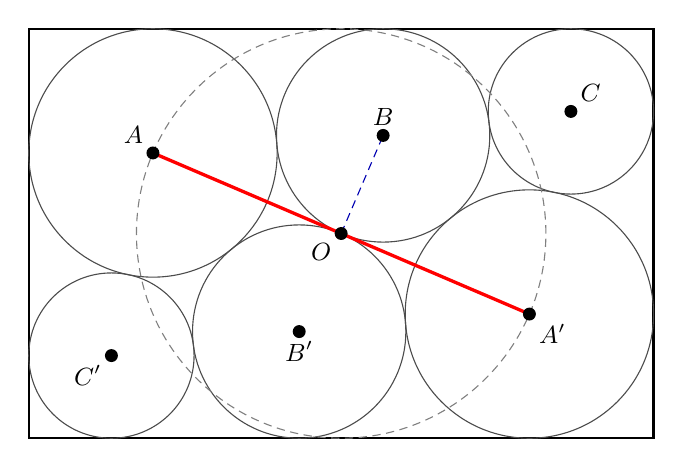
\begin{tikzpicture}[scale=2.6]
\draw[thick] (-1.5259,-1) rectangle (1.5259,1);
\draw[black!70] (-0.9194,0.3934) circle (0.6066);
\draw[black!70] (0.2050,0.4790) circle (0.5210);
\draw[black!70] (1.1222,0.5963) circle (0.4037);
\draw[black!70] (0.9194,-0.3934) circle (0.6066);
\draw[black!70] (-0.2050,-0.4790) circle (0.5210);
\draw[black!70] (-1.1222,-0.5963) circle (0.4037);
\draw[densely dashed, gray] (0,0) circle (1);
\draw[red, very thick] (-0.9194,0.3934) -- (0.9194,-0.3934);
\draw[densely dashed, blue!70!black] (0.0000,0.0000) -- (0.2050,0.4790);
\fill (0.0000,0.0000) circle (0.9pt) node[below left, font=\small] {$O$};
\fill (-0.9194,0.3934) circle (0.9pt) node[above left, font=\small] {$A$};
\fill (0.2050,0.4790) circle (0.9pt) node[above, font=\small] {$B$};
\fill (1.1222,0.5963) circle (0.9pt) node[above right, font=\small] {$C$};
\fill (0.9194,-0.3934) circle (0.9pt) node[below right, font=\small] {$A'$};
\fill (-0.2050,-0.4790) circle (0.9pt) node[below, font=\small] {$B'$};
\fill (-1.1222,-0.5963) circle (0.9pt) node[below left, font=\small] {$C'$};
\end{tikzpicture}

\caption{The top three circles touch the top side, $A$ and $C$ also touch the left and right sides, and $B$ passes through the centre $O$. The bottom three are the images of the top three under the half-turn about $O$. The dashed circle has centre $O$ and touches the top and bottom sides. The claim is that the red segment $AA'$ equals the height of the rectangle, or equivalently that $A$ lies on the dashed circle.}
\label{fig:config}
\end{figure}

Let the rectangle have centre $O$ and half-height $h$. Write $A$, $B$, $C$ for the centres of the top three circles, from left to right, and $a$, $b$, $c$ for their radii. Besides the contacts with the sides, the tangencies are: $B$ touches $A$, $C$ and $A'$, and $C$ touches $A'$. With $h=1$ one can compute $a\approx0.6066$, $b\approx0.5210$ and $c\approx0.4037$; the figures are drawn from this solution, though the proof never uses the numbers. We use only one feature of the picture that the tangencies do not spell out: each radius is less than $h$, so every centre in the top row lies above the horizontal through $O$.

\emph{Before reading on, try the first step.} Why is it enough to show that $OA=h$?

\textbf{The reduction.} Circle $B$ touches the congruent circles $A$ and $A'$, so $BA=BA'$. Since $O$ is the midpoint of $AA'$, the line $OB$ is the median of an isosceles triangle and so is perpendicular to $AA'$. The red segment is $2\,OA$, and it equals the height $2h$ exactly when $OA=h$. Call $\Omega$ the circle with centre $O$ and radius $h$, dashed in Figure~\ref{fig:config}. It touches the top side at its midpoint $U$, and the claim is that $A$ lies on $\Omega$.

\textbf{The plan.} Let $E'$ be the left end of the horizontal diameter of $\Omega$. If we knew that the line $AE'$ ran in a known direction, the triangle $OE'A$ would have one side $OE'=h$ and two known angles, and we could hope to show it is isosceles. The direction comes from the line $OB_t$, where $B_t$ is the point at which circle $B$ touches the top side. Steps 1 and 2 show that the line of centres $AC'$ is parallel to $OB_t$. Step 3 shows that this line passes through $E'$, and Step 4 finishes.

Put $\psi=\angle UOB_t$. In triangle $OBB_t$ the sides $BO$ and $BB_t$ are radii of circle $B$, and $BB_t$ is parallel to $OU$, so
\[
\angle UOB=2\psi ,
\]
twice the base angle. The point $B_t$ lies to the right of $U$: otherwise $A$ and $B$ would both lie above the horizontal through $O$ and on or to the left of $OU$, and the angle $AOB$ would be acute, contradicting the reduction.

\section*{1. A bisector}

One fact about tangent lengths does most of the work. Two circles of radii $r$ and $s$ that touch each other, and touch a line on the same side, touch the line at points $2\sqrt{rs}$ apart. (Their centres are $r+s$ apart and differ in height by $|r-s|$, and $(r+s)^2-(r-s)^2=4rs$.) For radii $1$ and $4$ the contact points are $4$ apart.

On the left side, $A$ and $C'$ touch each other and the side, at heights $h-a$ and $-(h-c)$, so $2h-a-c=2\sqrt{ac}$. On the top side, let $A_t$ and $C_t$ be the contact points of $A$ and $C$, so that $A_tC_t=2\sqrt{ab}+2\sqrt{bc}$. In short,
\begin{equation}\label{eq:tangent}
\sqrt a+\sqrt c=\sqrt{2h},\qquad A_tC_t=2\sqrt b\,(\sqrt a+\sqrt c).
\end{equation}
The first ties the two left-hand radii to the height. The second measures the top side between the corner contacts.

Circle $B$ passes through $O$ and touches the top side at $B_t$, so $B_t$ is one end of a vertical diameter of length $2b$. In the right-angled triangle formed by this diameter and $O$, the leg $OB_t$ satisfies $OB_t^2=2b\cdot h$, the diameter times the projection of the leg onto it. With~\eqref{eq:tangent},
\[
A_tC_t=2\sqrt{2bh}=2\,OB_t .
\]

Let $M$ be the midpoint of $A_tC_t$. Along the top side, $M$ lies $\tfrac12(a-c)$ to the right of $U$, because $A_t$ and $C_t$ are $a$ and $c$ in from the corners. And $B_t$ lies $2\sqrt{ab}-\sqrt b(\sqrt a+\sqrt c)=\sqrt b(\sqrt a-\sqrt c)$ to the right of $M$. Both displacements have the sign of $a-c$, and $B_t$ is to the right of $U$, so $a>c$ and the order along the top is $U$, $M$, $B_t$. The ratio in which $M$ divides $UB_t$ is
\[
\frac{UM}{MB_t}=\frac{\tfrac12(a-c)}{\sqrt b(\sqrt a-\sqrt c)}=\frac{\sqrt a+\sqrt c}{2\sqrt b}=\frac{h}{\sqrt{2bh}}=\frac{OU}{OB_t},
\]
using $a-c=(\sqrt a-\sqrt c)(\sqrt a+\sqrt c)$ and then~\eqref{eq:tangent}. By the converse of the angle bisector theorem in triangle $UOB_t$, the line $OM$ bisects the angle $UOB_t$.

\begin{figure}[ht]
\centering
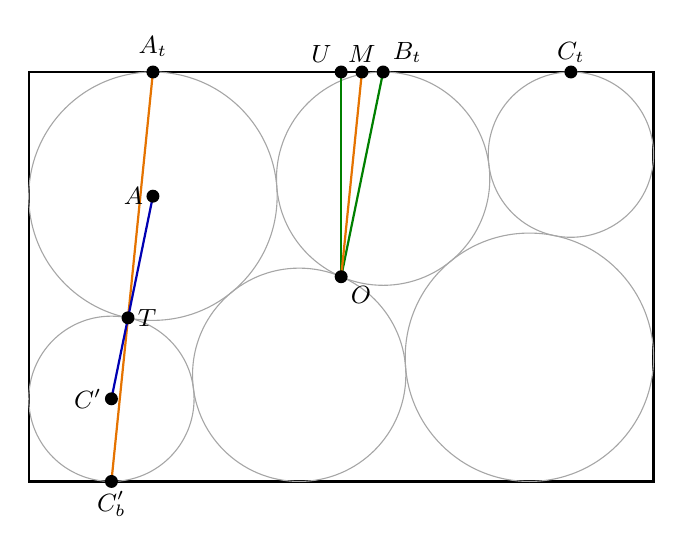
\begin{tikzpicture}[scale=2.6]
\draw[thick] (-1.5259,-1) rectangle (1.5259,1);
\draw[black!35] (-0.9194,0.3934) circle (0.6066);
\draw[black!35] (0.2050,0.4790) circle (0.5210);
\draw[black!35] (1.1222,0.5963) circle (0.4037);
\draw[black!35] (0.9194,-0.3934) circle (0.6066);
\draw[black!35] (-0.2050,-0.4790) circle (0.5210);
\draw[black!35] (-1.1222,-0.5963) circle (0.4037);
\draw[green!50!black, thick] (0.0000,0.0000) -- (0.0000,1.0000);
\draw[green!50!black, thick] (0.0000,0.0000) -- (0.2050,1.0000);
\draw[orange!90!black, thick] (0.0000,0.0000) -- (0.1014,1.0000);
\draw[orange!90!black, thick] (-0.9194,1.0000) -- (-1.1222,-1.0000);
\draw[blue!70!black, thick] (-0.9194,0.3934) -- (-1.1222,-0.5963);
\fill (0.0000,0.0000) circle (0.9pt) node[below right, font=\small] {$O$};
\fill (0.0000,1.0000) circle (0.9pt) node[above left, font=\small] {$U$};
\fill (0.1014,1.0000) circle (0.9pt) node[above, font=\small] {$M$};
\fill (0.2050,1.0000) circle (0.9pt) node[above right, font=\small] {$B_t$};
\fill (-0.9194,1.0000) circle (0.9pt) node[above=2pt, font=\small] {$A_t$};
\fill (1.1222,1.0000) circle (0.9pt) node[above, font=\small] {$C_t$};
\fill (-1.0412,-0.2008) circle (0.9pt) node[right, font=\small] {$T$};
\fill (-1.1222,-1.0000) circle (0.9pt) node[below, font=\small] {$C'_b$};
\fill (-0.9194,0.3934) circle (0.9pt) node[left, font=\small] {$A$};
\fill (-1.1222,-0.5963) circle (0.9pt) node[left, font=\small] {$C'$};
\end{tikzpicture}

\caption{Steps 1 and 2. The orange line $OM$ bisects the angle between the green lines $OU$ and $OB_t$. The orange line from $A_t$ through the contact point $T$ to $C'_b$ is parallel to it, and the blue line of centres $AC'$ is then parallel to $OB_t$.}
\label{fig:bisector}
\end{figure}

\section*{2. A parallel}

Step 1 gave a direction at $O$. To carry it to the line of centres $AC'$ we need a line through both circles $A$ and $C'$ whose direction we can read off, and a homothety between the two circles supplies one. Let $T$ be the point where circles $A$ and $C'$ touch, and let $C'_b$ be the lowest point of circle $C'$. The homothety with centre $T$ and negative ratio that maps circle $A$ to circle $C'$ maps the highest point $A_t$ of the first to the lowest point $C'_b$ of the second, so $A_t$, $T$ and $C'_b$ are collinear. From $A_t$ to $C'_b$ the horizontal and vertical separations are $a-c$ and $2h$, exactly twice those from $O$ to $M$. Hence $A_tT$ is parallel to $OM$ and makes the angle $\psi/2$ with the vertical. The triangle $AA_tT$ is isosceles with base angles $\psi/2$, so its angle at $A$ is $180^\circ-\psi$ and the radius $AT$ makes the angle $\psi$ with the downward vertical, and so does the line of centres $AC'$, which passes through $T$. Both $AC'$ and $OB_t$ rise to the right, so
\[
AC'\parallel OB_t .
\]

\section*{3. The line of centres passes through $E'$}

We now need to locate $AC'$, not just its direction, and the length to aim for is $h$. The circle $\Omega$ puts that length on the line $OB_t$. Let $K$ be the point where $OB_t$ crosses $\Omega$, so $OK=h$. It lies between $O$ and $B_t$, because $OB_t$ is the hypotenuse of the right-angled triangle $OUB_t$ and so is longer than $OU=h$. The tangents to $\Omega$ at $U$ and $K$ meet at a point on the bisector of the angle $UOK$, which is $OM$; the tangent at $U$ is the top side, so they meet at $M$. Hence $MK=MU$ and $MK\perp OB_t$ (Figure~\ref{fig:triangles}).

Now let $S$ be the midpoint of $AC'$ and $S_0$ the foot of the perpendicular from $S$ to the horizontal through $O$. The centres $A$ and $C'$ are $a$ and $c$ in from the left side, and the half-width of the rectangle is $\tfrac12(A_tC_t+a+c)$, so
\[
OS_0=\tfrac12A_tC_t=OB_t,\qquad SS_0=\tfrac12(a-c)=UM ,
\]
with $S_0$ to the left of $O$ and $S$ below it. In words: $S_0$ is as far from $O$ as $B_t$ is, and $S$ sits as far below the horizontal as $M$ sits to the right of $U$.

Let the line $AC'$ cross the horizontal through $O$ at $X$. Compare the right-angled triangles $MKB_t$ and $SS_0X$, shaded in Figure~\ref{fig:triangles}. Their legs $MK$ and $SS_0$ both equal $UM$. The angle at $M$ is $\psi$, because the angle at $B_t$ is $\angle OB_tU=90^\circ-\psi$. The angle at $S$ is also $\psi$, because $SX$ lies along $AC'$, which is parallel to $OB_t$. So the triangles are congruent, and
\[
S_0X=KB_t=OB_t-h .
\]
Going up $AC'$ from $S$ to the horizontal moves to the right, so $X$ lies to the right of $S_0$, at distance $OS_0-S_0X=h$ from $O$. That is, $X=E'$.

\begin{figure}[ht]
\centering
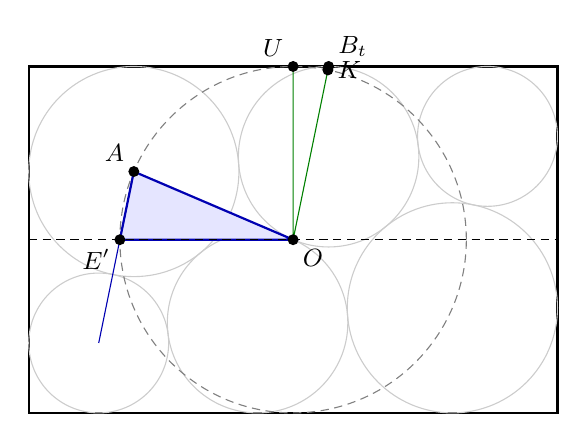
\begin{tikzpicture}[scale=2.2]
\draw[thick] (-1.5259,-1) rectangle (1.5259,1);
\draw[black!20] (-0.9194,0.3934) circle (0.6066);
\draw[black!20] (0.2050,0.4790) circle (0.5210);
\draw[black!20] (1.1222,0.5963) circle (0.4037);
\draw[black!20] (0.9194,-0.3934) circle (0.6066);
\draw[black!20] (-0.2050,-0.4790) circle (0.5210);
\draw[black!20] (-1.1222,-0.5963) circle (0.4037);
\draw[densely dashed, gray] (0,0) circle (1);
\filldraw[fill=blue!10, draw=blue!70!black, thick] (0.0000,0.0000) -- (-1.0000,0.0000) -- (-0.9194,0.3934) -- cycle;
\draw[green!50!black] (0.0000,0.0000) -- (0.0000,1.0000) (0.0000,0.0000) -- (0.2050,1.0000);
\draw[densely dashed] (-1.5259,0) -- (1.5259,0);
\draw[blue!70!black] (-0.9194,0.3934) -- (-1.1222,-0.5963);
\fill (0.0000,0.0000) circle (0.9pt) node[below right, font=\small] {$O$};
\fill (0.0000,1.0000) circle (0.9pt) node[above left, font=\small] {$U$};
\fill (0.2050,1.0000) circle (0.9pt) node[above right, font=\small] {$B_t$};
\fill (0.2008,0.9796) circle (0.9pt) node[right, font=\small] {$K$};
\fill (-1.0000,0.0000) circle (0.9pt) node[below left, font=\small] {$E'$};
\fill (-0.9194,0.3934) circle (0.9pt) node[above left, font=\small] {$A$};
\end{tikzpicture}
\qquad
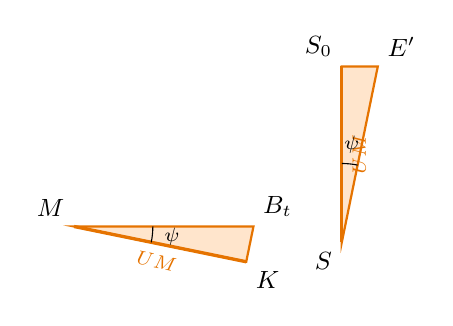
\begin{tikzpicture}
\coordinate (M) at (0.000,0.000);
\coordinate (K) at (2.186,-0.448);
\coordinate (Bt) at (2.278,0.000);
\filldraw[fill=orange!20, draw=orange!90!black, thick] (0.000,0.000) -- (2.186,-0.448) -- (2.278,0.000) -- cycle;
\draw[orange!90!black, very thick] (0.000,0.000) -- (2.186,-0.448) node[midway, sloped, below, font=\scriptsize] {$UM$};
\draw pic[draw, angle radius=10mm, "$\psi$", angle eccentricity=1.25, font=\scriptsize] {angle=K--M--Bt};
\node[above left, font=\small] at (0.000,0.000) {$M$};
\node[below right, font=\small] at (2.186,-0.448) {$K$};
\node[above right, font=\small] at (2.278,0.000) {$B_t$};
\coordinate (S) at (3.400,-0.200);
\coordinate (S0) at (3.400,2.032);
\coordinate (E) at (3.857,2.032);
\filldraw[fill=orange!20, draw=orange!90!black, thick] (3.400,-0.200) -- (3.400,2.032) -- (3.857,2.032) -- cycle;
\draw[orange!90!black, very thick] (3.400,-0.200) -- (3.400,2.032) node[midway, sloped, below, font=\scriptsize] {$UM$};
\draw pic[draw, angle radius=10mm, "$\psi$", angle eccentricity=1.25, font=\scriptsize] {angle=E--S--S0};
\node[below left, font=\small] at (3.400,-0.200) {$S$};
\node[above left, font=\small] at (3.400,2.032) {$S_0$};
\node[above right, font=\small] at (3.857,2.032) {$E'$};
\end{tikzpicture}

\caption{Steps 3 and 4. Left: the line of centres $AC'$ passes through $E'$, the left end of the horizontal diameter of $\Omega$, and the blue triangle $OE'A$ is isosceles. Right: the two small right triangles $MKB_t$ and $SS_0E'$, magnified 22 times at the same scale. Their thick legs both equal $UM$ and the marked angles are both $\psi$, so they are congruent.}
\label{fig:triangles}
\end{figure}

\section*{4. The isosceles triangle}

In triangle $OE'A$ the side $E'A$ lies along $AC'$, which is parallel to $OB_t$ and so makes the angle $90^\circ-\psi$ with the horizontal $E'O$. Turning the figure through a right angle about $O$ takes the upward vertical to the leftward horizontal and, since $OA\perp OB$, takes the line $OB$ to the line $OA$. So the angle $E'OA$ equals the angle $UOB=2\psi$. The three angles are
\[
\angle E'OA=2\psi,\qquad \angle OE'A=90^\circ-\psi,\qquad \angle OAE'=180^\circ-2\psi-(90^\circ-\psi)=90^\circ-\psi .
\]
The angles at $E'$ and $A$ are equal, so $OA=OE'=h$. The point $A$ lies on $\Omega$, and the red segment $AA'$ equals the height $2h$. \hfill$\square$

\textbf{Acknowledgements.} The problem and its history are due to Dan~\cite{MSE,MO}. A longer version of this proof first appeared as the author's answer on MathOverflow~\cite{MOA}. The author used AI tools in developing this proof and takes full responsibility for its content.

\begin{thebibliography}{9}
\bibitem{MSE} Dan, \emph{Six circles in a rectangle: show that two lengths are equal}, Mathematics Stack Exchange question 5112314 (4 December 2025), \url{https://math.stackexchange.com/q/5112314}.
\bibitem{MO} Dan, \emph{Six circles in a rectangle: show that two lengths are equal, using pure geometry}, MathOverflow question 515498 (24 September 2026), \url{https://mathoverflow.net/q/515498}.
\bibitem{MOA} V.~Jandhyala, answer to MathOverflow question 515498 (1 October 2026), \url{https://mathoverflow.net/a/515659}.
\end{thebibliography}

\bigskip
\noindent VAMSHI JANDHYALA\\
London, United Kingdom

\end{document}
